% --- Page Style ---
\pagestyle{fancy}
\fancyhf{}
\lhead{Algebra --- Unit 2}
\rhead{Exam ID: \underline{\hspace{2cm}}}
\lfoot{Simplified and exact. No calculators.}
\rfoot{Page \thepage}
\renewcommand{\headrulewidth}{0.4pt}
\renewcommand{\footrulewidth}{0.4pt}

% --- Header spanning both columns ---
\twocolumn[
  \begin{center}
    {\huge \textbf{Unit 2 Test}} \\
    \vgap
    {\large \textbf{Algebra}} \\
    \vgap
    \begin{tabular}{|l|l|}
      \hline
      \textbf{Student Name:} & \hspace{6cm} \\ \hline
      \textbf{Date:} & \hspace{6cm} \\ \hline
    \end{tabular}
  \end{center}
  \vgap
  \textbf{Instructions:} All answers on this assessment should be simplified and exact. No calculators are allowed.
  \vgap
]

% --- Form A (Questions 1--15) ---
\section*{Form A}

\begin{enumerate}[leftmargin=*, label=\textbf{\arabic*.}]

  \item Factor: $x^2 - 8x + 12$. \points{1}
  \vgap

  \item Factor: $6x^2 - 7x - 3$. \points{1}
  \vgappp

  \item Solve the equation for $x$ by completing the square. Note that $a$ is a constant and can appear in your answer. \points{5}
  \[
  3x^2 - 6ax = 4
  \]
  \vgappp

  \item Solve the equation for $x$: $2x^2 + 6x - 8 = 13x - 4$. \points{3}

  Answer: $x = $ \blank
  \vgappp

  \item If $h(x) = -3x^2 + 5bx + 2$ has two real roots, give all possible values of $b$. State your answer in interval notation. \points{3}
  \vgappp

  \item The function $f(x)$ is a quadratic with real coefficients and exactly one distinct real root. The graph of $f(x)$ intersects the line $y = \frac{9}{2}$ when $x = 1$ and again when $x = 5$. Graph $f(x)$ on the axes below. Be sure to include 3 points on the graph. \points{1}

  \begin{center}
  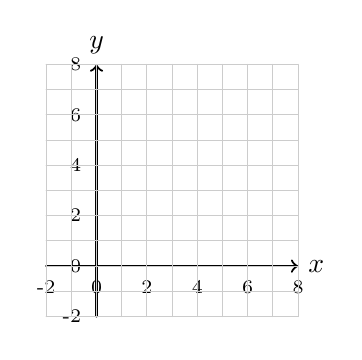
\begin{tikzpicture}[x=0.32cm, y=0.32cm, line cap=round, line join=round]
    \draw[thick,->] (-2,0) -- (8,0) node[right] {$x$};
    \draw[thick,->] (0,-2) -- (0,8) node[above] {$y$};
    \foreach \x in {-2,0,2,4,6,8} \draw (\x,2pt) -- (\x,-2pt) node[below,font=\scriptsize] {\x};
    \foreach \y in {-2,0,2,4,6,8} \draw (2pt,\y) -- (-2pt,\y) node[left,font=\scriptsize] {\y};
    \draw[gray!40] (-2,-2) grid[step=1] (8,8);
  \end{tikzpicture}
  \end{center}
  \vgapp

  \item Write $f(x)$ in vertex form. \points{2}
  \vgapp

  \item Write $f(x)$ in factored form. \points{1}
  \vgap

  \item Write $f(x)$ in standard form. \points{1}
  \vgappp

  \item Simplify: $\dfrac{60-14i}{-4i+6}$. \points{1}
  \vgappp

  \item Solve $4x^2 + x + 19 = x + 10$ by factoring. \points{3}
  \vgappp

  \item A quadratic function $f(x)$ has a root at $\dfrac{12i+8}{2i-3}$ and its graph contains the point $(2,40)$. Solve the inequality $f(x) \geq 47 - x$. Write your answer in interval notation. \points{4}
  \vgappp

  \item The graph of a function $f(x)$ is given on the axes below. Use the graph to write $f(x)$ in vertex form. \points{2}

  \begin{center}
  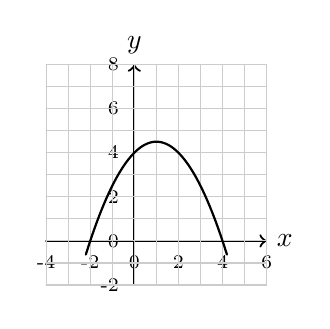
\begin{tikzpicture}[x=0.28cm, y=0.28cm, line cap=round, line join=round]
    \draw[thick,->] (-4,0) -- (6,0) node[right] {$x$};
    \draw[thick,->] (0,-2) -- (0,8) node[above] {$y$};
    \foreach \x in {-4,-2,0,2,4,6} \draw (\x,2pt) -- (\x,-2pt) node[below,font=\scriptsize] {\x};
    \foreach \y in {-2,0,2,4,6,8} \draw (2pt,\y) -- (-2pt,\y) node[left,font=\scriptsize] {\y};
    \draw[gray!40] (-4,-2) grid[step=1] (6,8);
    \draw[thick,domain=-2.2:4.2,samples=80] plot (\x, {-0.5*(\x-1)*(\x-1)+4.5});
  \end{tikzpicture}
  \end{center}
  \vgap

  \item Write $f(x)$ in factored form. \points{1}
  \vgap

  \item Write $f(x)$ in standard form. \points{1}
  \vgapp

\end{enumerate}

\clearpage
% --- Form B (Questions 16--30) ---
\section*{Form B}

\begin{enumerate}[leftmargin=*, label=\textbf{\arabic*.}, resume]

  \item Factor: $x^2 + 7x + 12$. \points{1}
  \vgap

  \item Factor: $9x^2 - 16x - 4$. \points{1}
  \vgappp

  \item Solve the equation for $x$ by completing the square. Note that $a$ is a constant and can appear in your answer. \points{5}
  \[
  2x^2 - 12ax = 2
  \]
  \vgappp

  \item Solve the equation for $x$: $4x^2 + 6x - 8 = 12x - 4$. \points{3}

  Answer: $x = $ \blank
  \vgappp

  \item If $h(x) = 3x^2 - 2bx + 2$ has two nonreal roots, give all possible values of $b$. State your answer in interval notation. \points{3}
  \vgappp

  \item The function $f(x)$ is a quadratic with real coefficients and exactly one distinct real root. The graph of $f(x)$ intersects the line $y = -1$ when $x = -1$ and again when $x = 7$. Graph $f(x)$ on the axes below. Be sure to include 3 points on the graph. \points{1}

  \begin{center}
  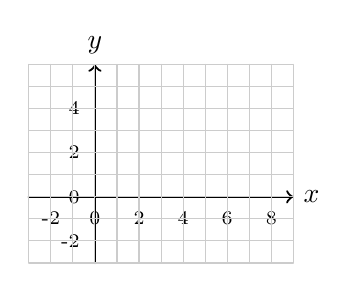
\begin{tikzpicture}[x=0.28cm, y=0.28cm, line cap=round, line join=round]
    \draw[thick,->] (-3,0) -- (9,0) node[right] {$x$};
    \draw[thick,->] (0,-3) -- (0,6) node[above] {$y$};
    \foreach \x in {-2,0,2,4,6,8} \draw (\x,2pt) -- (\x,-2pt) node[below,font=\scriptsize] {\x};
    \foreach \y in {-2,0,2,4} \draw (2pt,\y) -- (-2pt,\y) node[left,font=\scriptsize] {\y};
    \draw[gray!40] (-3,-3) grid[step=1] (9,6);
  \end{tikzpicture}
  \end{center}
  \vgapp

  \item Write $f(x)$ in vertex form. \points{2}
  \vgapp

  \item Write $f(x)$ in factored form. \points{1}
  \vgap

  \item Write $f(x)$ in standard form. \points{1}
  \vgappp

  \item Simplify: $\dfrac{10-4i}{-2i+1}$. \points{1}
  \vgappp

  \item Solve $16x^2 + 8x + 19 = 8x + 10$ by factoring. \points{3}
  \vgappp

  \item A quadratic function $f(x)$ has a root at $\dfrac{12i+6}{2i-4}$ and its graph contains the point $(3,54)$. Solve the inequality $f(x) < 5x + 35$. Write your answer in interval notation. \points{4}
  \vgappp

  \item The graph of a function $f(x)$ is given on the axes below. Use the graph to write $f(x)$ in vertex form. \points{2}

  \begin{center}
  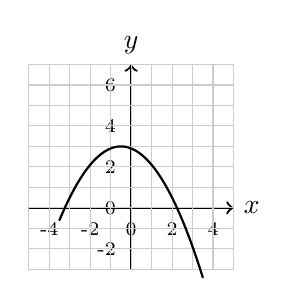
\begin{tikzpicture}[x=0.26cm, y=0.26cm, line cap=round, line join=round]
    \draw[thick,->] (-5,0) -- (5,0) node[right] {$x$};
    \draw[thick,->] (0,-3) -- (0,7) node[above] {$y$};
    \foreach \x in {-4,-2,0,2,4} \draw (\x,2pt) -- (\x,-2pt) node[below,font=\scriptsize] {\x};
    \foreach \y in {-2,0,2,4,6} \draw (2pt,\y) -- (-2pt,\y) node[left,font=\scriptsize] {\y};
    \draw[gray!40] (-5,-3) grid[step=1] (5,7);
    \draw[thick,domain=-3.5:3.5,samples=80] plot (\x, {-0.4*(\x+0.5)*(\x+0.5)+3});
  \end{tikzpicture}
  \end{center}
  \vgap

  \item Write $f(x)$ in factored form. \points{1}
  \vgap

  \item Write $f(x)$ in standard form. \points{1}
  \vgapp

\end{enumerate}

\clearpage
% --- Form C (Questions 31--45) ---
\section*{Form C}

\begin{enumerate}[leftmargin=*, label=\textbf{\arabic*.}, resume]

  \item Factor: $x^2 - 12x - 28$. \points{1}
  \vgap

  \item Factor: $3x^2 - 7x - 6$. \points{1}
  \vgappp

  \item Solve the equation for $x$ by completing the square. Note that $a$ is a constant and can appear in your answer. \points{5}
  \[
  2x^2 + 8ax = 5
  \]
  \vgappp

  \item Solve the equation for $x$: $3x^2 + 6x - 8 = 13x - 10$. \points{3}

  Answer: $x = $ \blank
  \vgappp

  \item If $h(x) = -2x^2 - 7bx - 1$ has two nonreal roots, give all possible values of $b$. State your answer in interval notation. \points{3}
  \vgappp

  \item The function $f(x)$ is a quadratic with real coefficients and exactly one distinct real root. The graph of $f(x)$ intersects the line $y = -4$ when $x = -4$ and again when $x = 0$. Graph $f(x)$ on the axes below. Be sure to include 3 points on the graph. \points{1}

  \begin{center}
  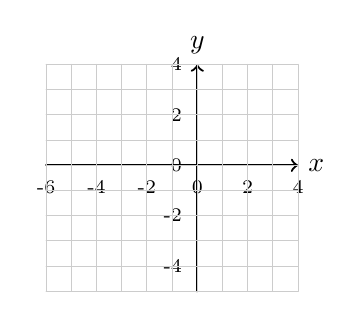
\begin{tikzpicture}[x=0.32cm, y=0.32cm, line cap=round, line join=round]
    \draw[thick,->] (-6,0) -- (4,0) node[right] {$x$};
    \draw[thick,->] (0,-5) -- (0,4) node[above] {$y$};
    \foreach \x in {-6,-4,-2,0,2,4} \draw (\x,2pt) -- (\x,-2pt) node[below,font=\scriptsize] {\x};
    \foreach \y in {-4,-2,0,2,4} \draw (2pt,\y) -- (-2pt,\y) node[left,font=\scriptsize] {\y};
    \draw[gray!40] (-6,-5) grid[step=1] (4,4);
  \end{tikzpicture}
  \end{center}
  \vgapp

  \item Write $f(x)$ in vertex form. \points{2}
  \vgapp

  \item Write $f(x)$ in factored form. \points{1}
  \vgap

  \item Write $f(x)$ in standard form. \points{1}
  \vgappp

  \item Simplify: $\dfrac{6-4i}{3i-5}$. \points{1}
  \vgappp

  \item Solve $9x^2 + 2x + 9 = 2x + 5$ by factoring. \points{3}
  \vgappp

  \item A quadratic function $f(x)$ has a root at $\dfrac{2-10i}{i+5}$ and its graph contains the point $(3,26)$. Solve the inequality $f(x) \leq 12 + 7x$. Write your answer in interval notation. \points{4}
  \vgappp

  \item The graph of a function $f(x)$ is given on the axes below. Use the graph to write $f(x)$ in vertex form. \points{2}

  \begin{center}
  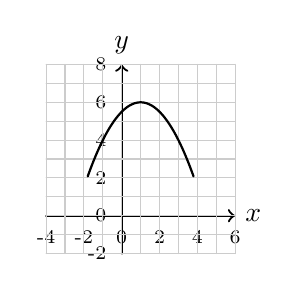
\begin{tikzpicture}[x=0.24cm, y=0.24cm, line cap=round, line join=round]
    \draw[thick,->] (-4,0) -- (6,0) node[right] {$x$};
    \draw[thick,->] (0,-2) -- (0,8) node[above] {$y$};
    \foreach \x in {-4,-2,0,2,4,6} \draw (\x,2pt) -- (\x,-2pt) node[below,font=\scriptsize] {\x};
    \foreach \y in {-2,0,2,4,6,8} \draw (2pt,\y) -- (-2pt,\y) node[left,font=\scriptsize] {\y};
    \draw[gray!40] (-4,-2) grid[step=1] (6,8);
    \draw[thick,domain=-1.8:3.8,samples=80] plot (\x, {-0.5*(\x-1)*(\x-1)+6});
  \end{tikzpicture}
  \end{center}
  \vgap

  \item Write $f(x)$ in factored form. \points{1}
  \vgap

  \item Write $f(x)$ in standard form. \points{1}
  \vgapp

\end{enumerate}
